\documentclass[10pt,a4paper]{article}
\usepackage[margin=1.9cm,top=1.7cm,bottom=1.8cm]{geometry}
\usepackage{amsmath,amssymb}
\usepackage{graphicx}
\usepackage{booktabs}
\usepackage[table]{xcolor}
\usepackage{microtype}
\usepackage{caption}
\usepackage{enumitem}
\usepackage[colorlinks=true,linkcolor=blue!50!black,citecolor=green!40!black,urlcolor=blue!60!black]{hyperref}
\captionsetup{font=small,labelfont=bf}
\setlist{itemsep=1pt,topsep=2pt}
\graphicspath{{../figures/}}
\newcommand{\sq}{\sqrt{f_R}}
\newcommand{\dd}{\mathrm{d}}
\newcommand{\RR}{\mathcal R}
\newcommand{\TT}{\mathcal T}
\definecolor{idea}{RGB}{42,120,214}
\newcommand{\idea}[1]{\par\smallskip\noindent\colorbox{idea!8}{\parbox{\dimexpr\linewidth-2\fboxsep}{\small\textbf{\color{idea}Idea.} #1}}\par\smallskip}

\title{\vspace{-8mm}\textbf{Gravitational waves scattering off a spherical thin shell}\\[2pt]
\large Summary of the project: junction conditions, reflectivity, quasinormal modes and stability}
\author{Final project, gravitational-wave course}
\date{September 2026}

\begin{document}
\maketitle
\vspace{-6mm}

\begin{abstract}\noindent
A thin spherical shell of matter at radius $R>2M$ separates a flat interior from a Schwarzschild exterior of mass $M$.
It is the simplest horizonless compact object. We compute, for odd (axial) and even (polar) gravitational
perturbations, the reflection and transmission coefficients $\RR(\omega)$ and $\TT(\omega)$ and the quasinormal-mode (QNM)
spectrum. The first step is to find a background that can be static at all. A domain wall cannot be; a fluid shell
with a specific positive pressure can. For odd parity the shell then turns out to be a repulsive $\delta$-function in
the wave equation. For even parity it is a flux-conserving $2\times2$ transfer matrix. The shell is opaque at low
frequency and transparent at high frequency, and it approaches the black-hole reflectivity as $R\to2M$. Its ringing is
completely different from a black hole's, with long-lived trapped modes for $R<3M$. One even-parity mode of the
shell's own matter grows exponentially, so the static shell is unstable, in agreement with Pitre, Schneider and Poisson
(2026). Units: $G=c=1$, time dependence $e^{-i\omega t}$.
\end{abstract}

\section{The problem and the first obstacle: is there a static shell?}
Inside the shell, Birkhoff's theorem and regularity at $r=0$ force flat space: $\dd s^2=-\dd T^2+\dd r^2+r^2\dd\Omega^2$.
Outside, $\dd s^2=-f\,\dd t^2+f^{-1}\dd r^2+r^2\dd\Omega^2$ with $f=1-2M/r$. The shell carries a surface stress tensor
$S_{ab}=\sigma u_au_b+p\,(h_{ab}+u_au_b)$. Gluing the two geometries is governed by the Israel junction conditions
\cite{Israel66,Poisson04}:
\begin{equation}
[h_{ab}]=0,\qquad [K_{ab}]-h_{ab}[K]=-8\pi S_{ab},\qquad [X]\equiv X_+-X_- ,
\label{eq:israel}
\end{equation}
where $h_{ab}$ is the induced metric and $K_{ab}$ the extrinsic curvature. For a spherical shell $r=R(\tau)$ they give
the mass formula and the equation of motion (Ipser \& Sikivie \cite{IS84}, Eqs.~3.7--3.9):
\begin{equation}
\sigma=\frac{\sqrt{1+\dot R^2}-\sqrt{f(R)+\dot R^2}}{4\pi R},\qquad
(\alpha+\beta)\ddot R=-\frac{\alpha M}{R^2}+\frac{2p}{\sigma}\frac{\alpha\beta(\alpha+\beta)}{R},
\end{equation}
with $\alpha=\sqrt{1+\dot R^2}$ and $\beta=\sqrt{f+\dot R^2}$.

\idea{A monochromatic scattering problem ($e^{-i\omega t}$) needs a time-independent background. Before any wave
calculation we must therefore ask whether the shell can sit still.}

Gravity always pulls inward ($-\alpha M/R^2$). Pressure pushes outward only if $p>0$. Setting $\dot R=\ddot R=0$ gives a unique
answer:
\begin{equation}
\frac{p}{\sigma}=\kappa(R)=\frac{1-\sq}{4\sq}>0,\qquad \sigma=\frac{1-\sq}{4\pi R}.
\label{eq:kappa}
\end{equation}
This leads to four candidate models:
\begin{itemize}
\item \textbf{Domain wall} ($p=-\sigma$, the object of the prior notes). $\ddot R<0$ always, so it collapses to a black
hole \cite{IS84}. It can only be \emph{frozen} at its turning point (\emph{model A}), where $\ddot R=-(1+3\sq)/2R$.
\item \textbf{Dust} ($p=0$). It is not static either: $(\alpha+\beta)\ddot R=-\alpha M/R^2<0$.
\item \textbf{Static perfect fluid} with $p=\kappa(R)\sigma$ (\emph{model C}, the primary model). The pressure ratio
is fixed by the compactness, not free. The energy condition $p\le\sigma$ requires $R\ge25M/12$. For the perturbed shell
we need an equation of state, $\delta p=\Gamma\,\frac{p}{\sigma+p}\,\delta\sigma$ with $\Gamma=2$, as in
\cite{PSP26}.
\item \textbf{Gravastar} (de Sitter interior \cite{Pani09}). Not treated.
\end{itemize}
The interior clock runs slower: $\dd T=\sq\,\dd t$. A wave of frequency $\omega$ outside therefore has frequency
$\nu=\omega/\sq$ inside.

\section{Waves on each side and the junction conditions}
\idea{Away from the shell everything is textbook. Outside, the Regge--Wheeler/Zerilli equations hold; inside, the flat
wave equation. \emph{All} the physics of the shell is in how the two solutions are glued at $r=R$.}

We use the gauge-invariant master functions of Martel and Poisson \cite{MP05}: Cunningham--Price--Moncrief for odd
parity and Zerilli--Moncrief for even parity. Outside,
$\Psi_{,r_*r_*}+[\omega^2-V]\Psi=0$, with $V_{\rm RW}=f[\ell(\ell+1)/r^2-6M/r^3]$ \cite{RW57} or the Zerilli potential
$V_{\rm Z}$ \cite{Zerilli70}. Inside, $\Psi''+[\nu^2-\ell(\ell+1)/r^2]\Psi=0$. Its regular solution is the Riccati--Bessel
function $\hat\jmath_\ell(\nu r)$. In a global tortoise coordinate $x$ ($x=r_*$ outside, $\dd x=\dd r/\sq$ inside) the
whole problem is a 1D wave equation with the potential of Fig.~\ref{fig:pot}.

The linearized Israel equations~\eqref{eq:israel} were derived from first principles. On each side the metric
perturbation is written in its own Regge--Wheeler gauge. Because those gauges are not adapted to the shell, the shell's
position is described by perturbed embeddings, with radial displacements $\xi_\pm$ that differ on the two sides. The
metric perturbations are then expressed through the master functions. The derivation was done symbolically (SymPy)
and verified. The results are the following.

\textbf{Odd parity: a $\delta$-barrier.} Odd perturbations do not move the shell or its matter. The background term
$[K]^{(0)}$, flagged in the prior notes as the missing step, cancels exactly against the pressure term. What remains is
\begin{equation}
\Psi_+=\Psi_-,\qquad \Big[\frac{\dd\Psi}{\dd x}\Big]=\Delta\,\Psi,\qquad
\Delta=\frac{\sq(1-\sq)}{R}=4\pi\sigma\sq>0 .
\label{eq:odd}
\end{equation}
The shell acts on axial waves as a repulsive $\delta(x-x_R)$ potential. Its strength does not depend on $\omega$, on the
equation of state, or on whether the shell is a wall or a fluid. The same condition was recovered independently by
letting a smooth anisotropic shell become thin; the mismatch vanishes linearly in the thickness (Fig.~\ref{fig:thick}). It also agrees with
\cite{PSP26} and with the matching conditions of \cite{Pani09}.

\textbf{Even parity: a $2\times2$ transfer matrix.} Polar perturbations move the shell radially and make its fluid
oscillate. After eliminating the shell variables ($\xi_\pm$, $\delta\sigma$, velocity) one gets
\begin{equation}
\begin{pmatrix}\Psi_+\\ \Psi_+'\end{pmatrix}_{R}=\mathsf T(\omega;\ell,R/M,\Gamma)\begin{pmatrix}\Psi_-\\ \Psi_-'\end{pmatrix}_{R},
\qquad \det\mathsf T=f_R^{-1/2}\ \text{(exactly)} .
\end{equation}
$\Psi$ itself jumps across the shell, and $\mathsf T$ depends on frequency, with poles on the matter scale
$\omega\sim(M/R^3)^{1/2}$. The determinant identity was not imposed; it is what guarantees energy conservation, and it
holds to machine precision.

\begin{figure}[t]\centering
\begin{minipage}{0.49\textwidth}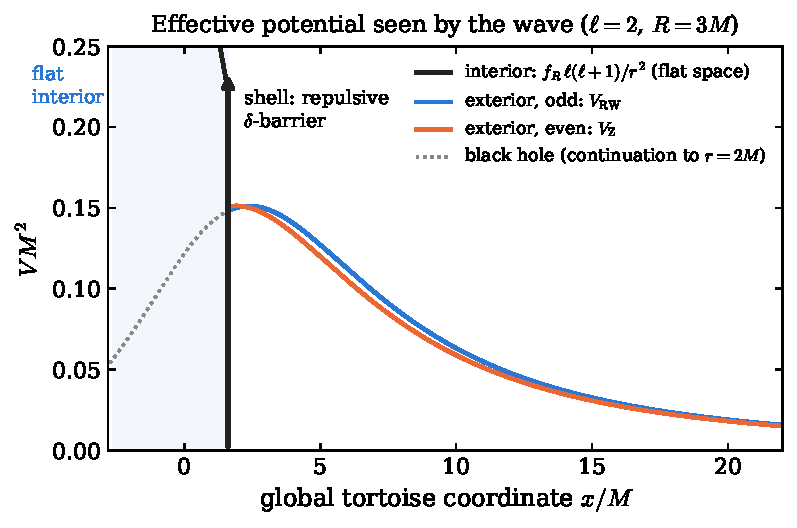
\includegraphics[width=\linewidth]{r3_f01_potential.pdf}
\caption{Potential seen by the wave. Flat interior (centrifugal barrier), shell ($\delta$-barrier, arrow) and
exterior RW/Zerilli barrier.}\label{fig:pot}\end{minipage}\hfill
\begin{minipage}{0.49\textwidth}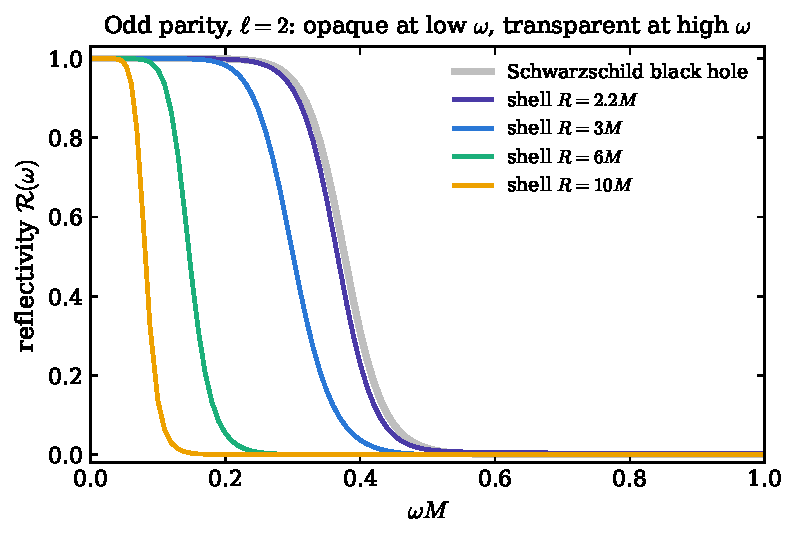
\includegraphics[width=\linewidth]{r3_f02_reflectivity_odd.pdf}
\caption{Reflectivity for odd parity, $\ell=2$. Compact shells approach the black-hole curve.}\label{fig:R}\end{minipage}
\end{figure}

\section{Scattering: how to define $\RR$ and $\TT$, and what they are}
\idea{Nothing is absorbed, so the \emph{closed} system reflects everything: $|B_{\rm out}/B_{\rm in}|=1$. To ask how much
the object reflects, we \emph{open} the interior. A wave that crosses the shell is let go (only the ingoing Hankel wave
$\hat h^{\rm in}_\ell(\nu r)$ inside), exactly as a horizon lets it go for a black hole.}

Outside, $\Psi\to B_{\rm in}e^{-i\omega r_*}+B_{\rm out}e^{i\omega r_*}$, and we define $\RR=|B_{\rm out}/B_{\rm in}|^2$
and $\TT=1/|B_{\rm in}|^2$. Flux conservation through the junction then implies $\RR+\TT=1$. Figures~\ref{fig:R}--\ref{fig:hf}
show four regimes:
\begin{itemize}
\item \textbf{Low frequency}: $\RR\to1$. Long waves are reflected, as for any compact object \cite{Boyanov25}.
\item \textbf{High frequency}: the potentials become negligible and only the $\delta$-barrier is left. Then
$\RR\simeq\Delta^2/(4\omega^2+\Delta^2)\to0$: \emph{the thin shell is transparent}. Even parity (model C) follows the
same law, because the fluid's inertia no longer matters (Fig.~\ref{fig:hf}).
\item \textbf{Compact shells, $R\to2M$}: $\Delta\to0$ and the shell sits deep in the redshifted throat, so
$\RR\to\RR_{\rm BH}$ (Vishveshwara \cite{Vishveshwara70}). The approach is slow, $\propto(R-2M)^{1/2}$.
\item \textbf{Dilute shells}: the transition to transparency happens at $\omega R\sim\ell$, set by the flat-space
centrifugal barrier.
\end{itemize}
Even and odd reflectivities differ at intermediate frequencies. The shell breaks the isospectrality of Schwarzschild.

\section{Quasinormal modes: how the shell rings}
QNMs are the complex $\omega$ at which the regular interior solution, carried through the junction, is purely outgoing
at infinity. They are found as zeros of a Wronskian. The outgoing solution comes from a Leaver-type continued fraction
\cite{Leaver85,Pani09} and independently from inward integration along a complex ray \cite{Boyanov25}. Three families
appear (Figs.~\ref{fig:qnm}, \ref{fig:matter}):
\begin{enumerate}
\item \textbf{Wave modes} of the interior cavity, with $\omega\sim1/R$. For dilute shells
${\rm Re}(\omega R)\approx n\pi$ and ${\rm Im}(\omega R)\approx-\tfrac12\ln[2\ell(\ell+1)R/M]$ \cite{PSP26}. The cavity leaks
through a weakly reflecting wall, so the damping is large and grows only logarithmically with $R$.
\item \textbf{Trapped modes} for $R<3M$, between the flat interior and the exterior photon-sphere barrier. They are damped
only by tunnelling and become extremely long-lived as $R\to2M$: ${\rm Im}\,\omega M\approx-10^{-6}$ at $R=2.01M$. These
are the modes behind gravitational-wave \emph{echoes} \cite{Cardoso2016PRL}. \emph{None of them tends to a Schwarzschild QNM},
even though the reflectivity does tend to the black-hole one.
\item \textbf{Matter modes} (even parity, model C only): oscillations of the shell itself, four per $\ell$, with
$\omega\sim(M/R^3)^{1/2}$. One of them is purely imaginary with ${\rm Im}\,\omega>0$.
\end{enumerate}

\begin{figure}[t]\centering
\begin{minipage}{0.49\textwidth}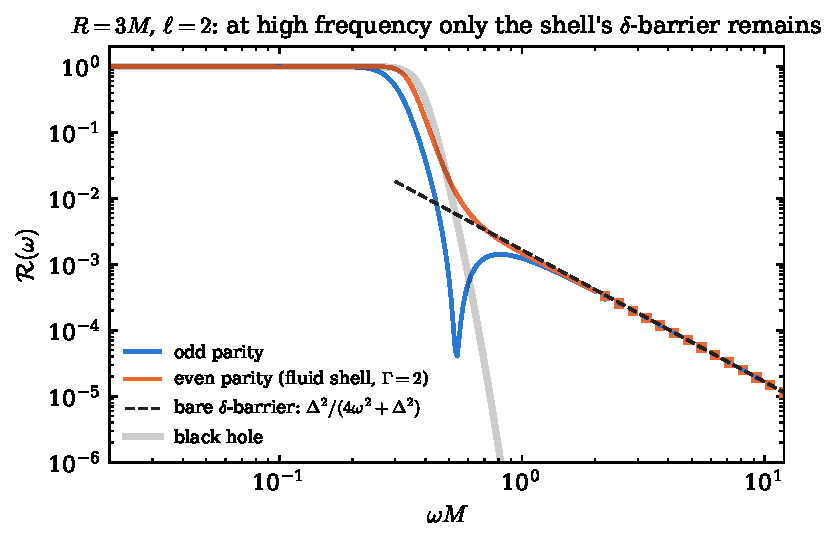
\includegraphics[width=\linewidth]{r3_f03_highfreq_law.pdf}
\caption{Odd and even ($\Gamma=2$) reflectivity at $R=3M$ on log axes, with the $\delta$-barrier law. Dots: points
computed up to $\omega M=12$.}\label{fig:hf}\end{minipage}\hfill
\begin{minipage}{0.49\textwidth}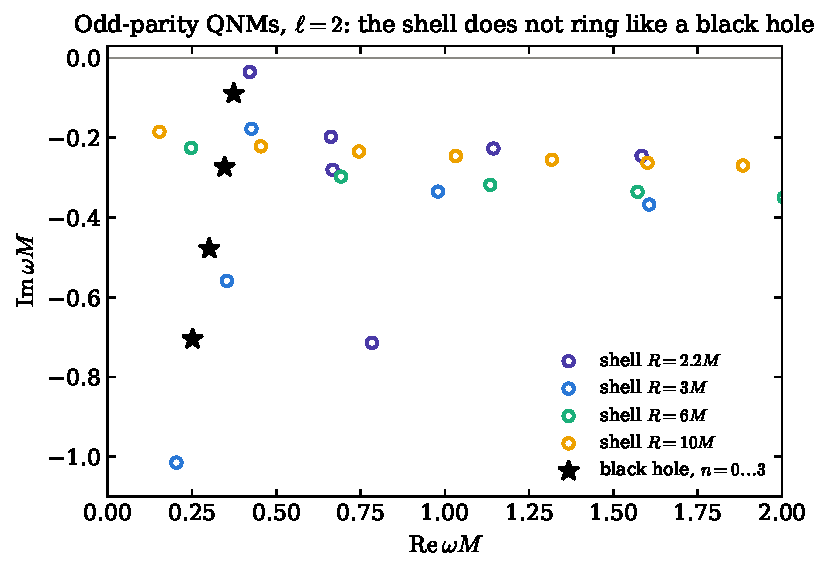
\includegraphics[width=\linewidth]{r3_f05_qnm_plane.pdf}
\caption{Odd QNMs ($\ell=2$) for four compactnesses, against the Schwarzschild modes (stars).}\label{fig:qnm}\end{minipage}
\end{figure}

\section{The static shell is unstable}
\idea{The only static member of the family, model C, should be stable if scattering off it is to describe
something physical. The growing matter mode shows that it is not. It is then essential to compare time scales.}

At $M/R=0.2$, $\ell=2$, $\Gamma=2$ the growing mode is $\omega(R^3/M)^{1/2}=0.6077\,i$, and the oscillating pair is
$1.2671-0.0011i$. These values agree with Pitre, Schneider and Poisson \cite{PSP26} at every compactness
(Fig.~\ref{fig:matter}), although their method (retarded-time slicing, spectral solver) is completely different. As
$M/R\to0$ they tend to the oscillations of a \emph{Newtonian} self-gravitating fluid shell. We derived that problem
from scratch; it gives $\varsigma^4-S\varsigma^2+P=0$ with $\varsigma^2=\omega^2R^3/M$, and for $\ell=2$ the roots are
$1.5050$ and $0.5147\,i$. The instability is therefore Newtonian in origin: the tangential pressure that holds the shell
up makes $\ell\ge2$ deformations run away. The same derivation shows that the constant term of the quartic in
\cite{PSP26}, Eq.~(7.6), contains a misprint; their closed form, Eq.~(7.8), is correct.

\textbf{Consequence for the models (Fig.~\ref{fig:time}).} The fluid shell grows on $\sim1.6(R^3/M)^{1/2}$, which is much
longer than the wave periods ($\sim R$). Scattering off model C is therefore a meaningful adiabatic idealization. The
domain wall collapses on $\omega_{\rm dyn}^{-1}\approx R/\sqrt2$, the light-crossing time, which is comparable to
the wave periods. For the frozen wall (model A) the even-parity junction system is overdetermined and inconsistent
(8 equations, 6 unknowns). Which two Israel equations are dropped is a free choice, and different choices change
$\RR$ at $O(1)$, from total reflection to the $\delta$-law (Fig.~\ref{fig:A}). \textbf{The even-parity results of model A are not
predictive}; its odd sector is identical to model C's.

\begin{figure}[t]\centering
\begin{minipage}{0.49\textwidth}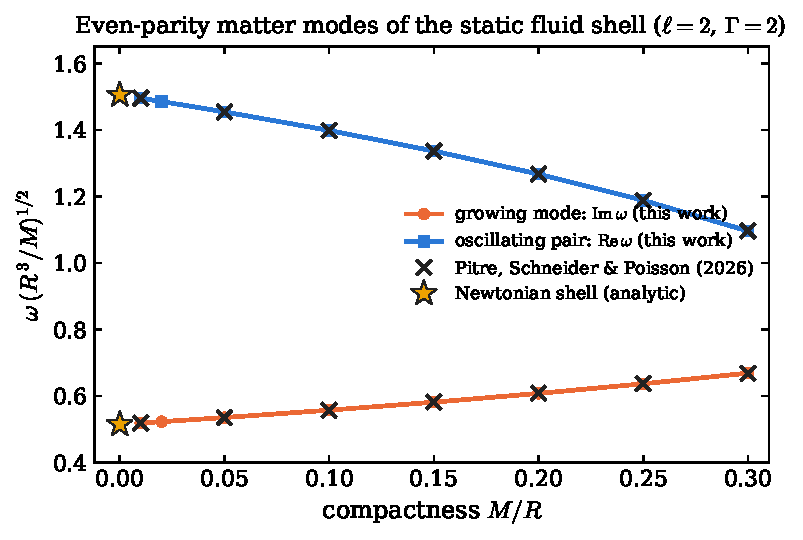
\includegraphics[width=\linewidth]{r3_f06_matter_modes.pdf}
\caption{Matter modes of the fluid shell vs compactness: growing mode (orange) and oscillating pair (blue). Crosses:
\cite{PSP26}. Stars: Newtonian shell.}\label{fig:matter}\end{minipage}\hfill
\begin{minipage}{0.49\textwidth}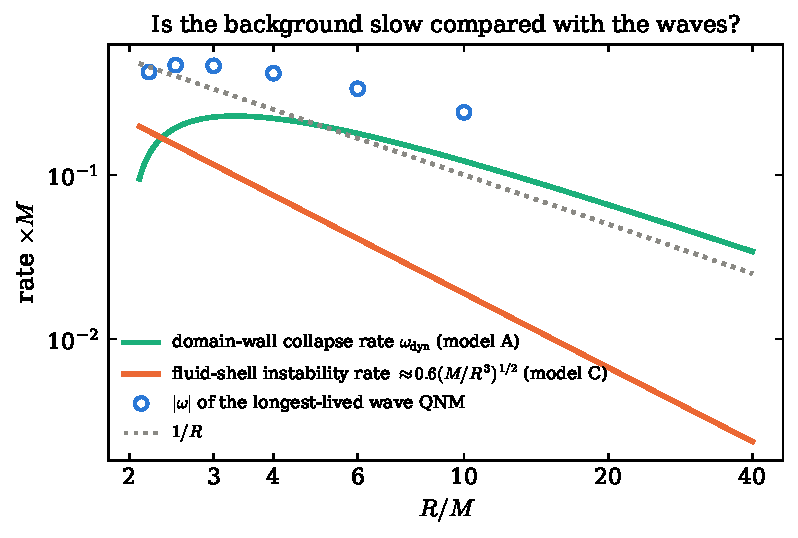
\includegraphics[width=\linewidth]{r3_f07_timescales.pdf}
\caption{Background rates vs the least-damped wave QNM. The wall collapses as fast as the waves oscillate; the fluid
instability is slow.}\label{fig:time}\end{minipage}
\end{figure}

\begin{figure}[ht]\centering
\begin{minipage}{0.49\textwidth}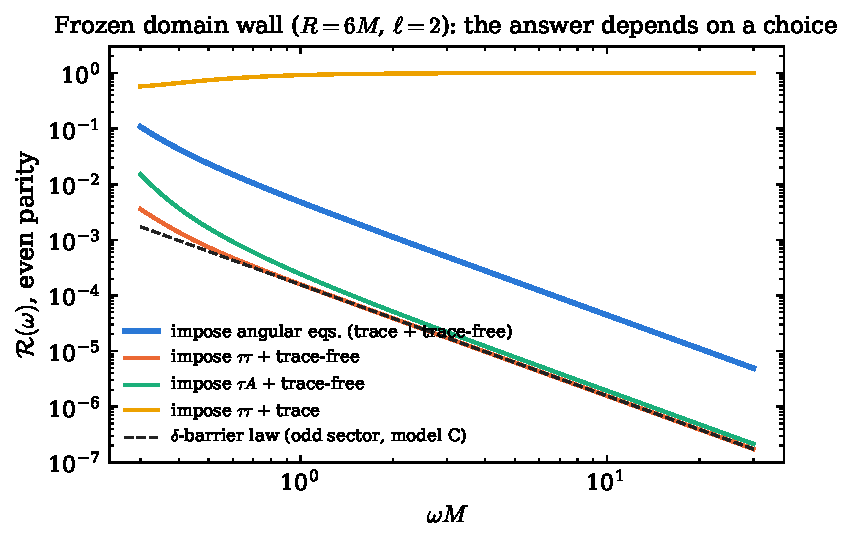
\includegraphics[width=\linewidth]{r3_f10_modelA_ambiguity.pdf}
\caption{Frozen domain wall, even parity: four equally defensible choices of which Israel equations to impose give
different $\RR(\omega)$.}\label{fig:A}\end{minipage}\hfill
\begin{minipage}{0.49\textwidth}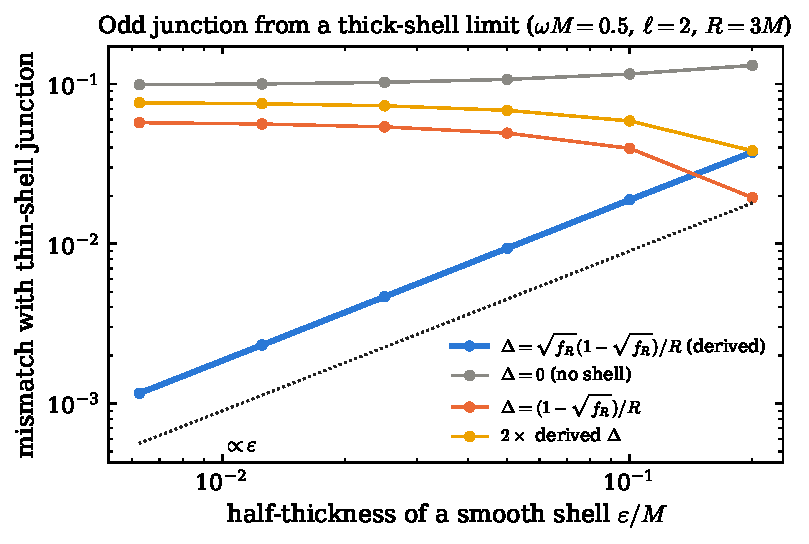
\includegraphics[width=\linewidth]{r3_f09_thick_shell.pdf}
\caption{Independent test of the odd junction: a smooth shell of half-thickness $\varepsilon$ converges to
Eq.~\eqref{eq:odd} and to no alternative.}\label{fig:thick}\end{minipage}
\end{figure}

\section{How we know it is right}
\begin{table}[h]\centering\small
\begin{tabular}{ll}\toprule
test & result\\\midrule
energy balance $|\RR+\TT-1|$ (odd, even model C, $\omega M\le2$) & $\lesssim6\times10^{-10}$\\
transfer matrix vs direct shooting, $\RR$ and $\TT$ & $\lesssim10^{-9}$\\
transfer matrix vs shooting, QNMs (397 modes) & median $\sim10^{-11}$, worst $6\times10^{-5}$\\
Schwarzschild $\ell=2$, $n=0$ (Leaver) & $0.3736716844-0.0889623157i$ \cite{BCS09}\\
black-hole reflectivity at $(2M\omega)^2=1$ & $1.55\times10^{-2}$, as in \cite{Vishveshwara70}\\
WKB orders 1, 3, 6 vs exact ($\ell=2$, $n=0$) & relative errors $7\%$, $0.15\%$, $0.02\%$ \cite{IW87,Konoplya03}\\
odd junction from a thick-shell limit & converges $\propto$ thickness\\
$\det\mathsf T\,\sq=1$ (even, model C) & to $10^{-12}$\\
time-domain ringdown vs QNM, $R=2.2M$ & $0.4215-0.0352i$ vs $0.4211-0.0350i$\\
time-domain ringdown vs QNM, black hole & $0.3731-0.0885i$ vs $0.3737-0.0890i$\\\bottomrule
\end{tabular}
\end{table}

\begin{figure}[h]\centering
\begin{minipage}{0.49\textwidth}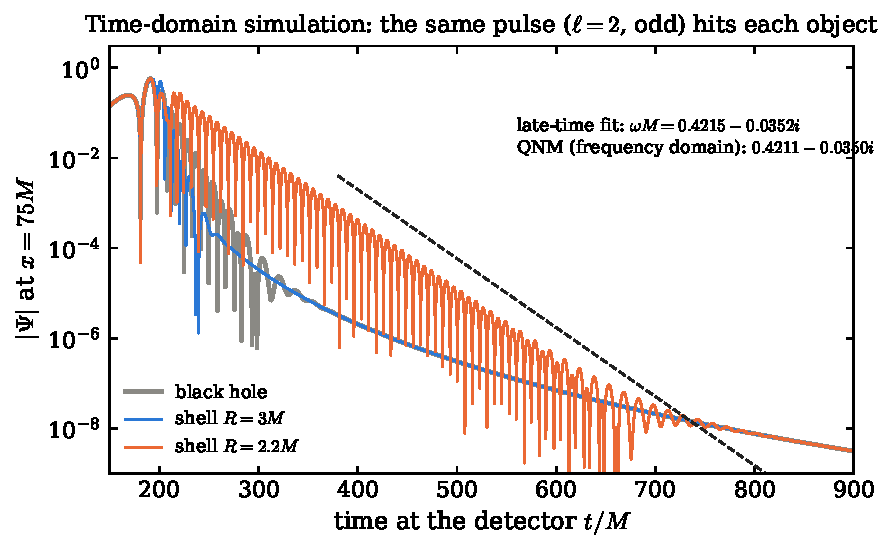
\includegraphics[width=\linewidth]{r3_f11_timedomain.pdf}\end{minipage}\hfill
\begin{minipage}{0.49\textwidth}
\caption{Time-domain simulation (odd, $\ell=2$). The same pulse is sent onto a black hole and onto two shells, and the
signal is recorded at $x=75M$. The black hole rings down quickly. The $R=2.2M$ shell keeps ringing at the frequency of
its trapped QNM, found independently in the frequency domain. All curves end in the same late-time power-law tail of
the exterior Schwarzschild potential.}\label{fig:td}\end{minipage}
\end{figure}

\section{Conclusions}
\begin{enumerate}
\item A thin shell with a flat interior is static only if it has positive surface pressure,
$p=\sigma(1-\sq)/4\sq$. Domain walls and dust shells collapse.
\item For axial waves the shell is a repulsive $\delta$-potential, $\Delta=\sq(1-\sq)/R$. For polar waves it is a
frequency-dependent, flux-conserving $2\times2$ transfer matrix, which also contains the dynamics of the shell's matter.
\item $\RR(\omega)$ goes from total reflection at low frequency to transparency at high frequency ($\RR\propto\omega^{-2}$).
It approaches the black-hole reflectivity as $R\to2M$, while the QNM spectrum does not approach the black-hole one.
Compact shells trap long-lived modes, which produce echoes.
\item The static shell is dynamically unstable through a Newtonian-origin matter mode. The instability is slow compared
with the waves, so the scattering results for the fluid shell are physically meaningful. The frozen domain wall is not
a controlled approximation in the even sector.
\end{enumerate}

\vspace{-2mm}
{\footnotesize
\begin{thebibliography}{99}\setlength{\itemsep}{0pt}
\bibitem{RW57} T.~Regge, J.~A.~Wheeler, Phys.\ Rev.\ \textbf{108}, 1063 (1957).
\bibitem{Zerilli70} F.~J.~Zerilli, Phys.\ Rev.\ Lett.\ \textbf{24}, 737 (1970).
\bibitem{Vishveshwara70} C.~V.~Vishveshwara, Nature \textbf{227}, 936 (1970).
\bibitem{Israel66} W.~Israel, Nuovo Cimento B \textbf{44}, 1 (1966).
\bibitem{IS84} J.~Ipser, P.~Sikivie, Phys.\ Rev.\ D \textbf{30}, 712 (1984).
\bibitem{Poisson04} E.~Poisson, \emph{A Relativist's Toolkit} (CUP, 2004), Ch.~3.
\bibitem{MP05} K.~Martel, E.~Poisson, Phys.\ Rev.\ D \textbf{71}, 104003 (2005).
\bibitem{Leaver85} E.~W.~Leaver, Proc.\ R.\ Soc.\ Lond.\ A \textbf{402}, 285 (1985).
\bibitem{IW87} S.~Iyer, C.~M.~Will, Phys.\ Rev.\ D \textbf{35}, 3621 (1987).
\bibitem{Konoplya03} R.~A.~Konoplya, Phys.\ Rev.\ D \textbf{68}, 024018 (2003).
\bibitem{BCS09} E.~Berti, V.~Cardoso, A.~O.~Starinets, Class.\ Quantum Grav.\ \textbf{26}, 163001 (2009).
\bibitem{Pani09} P.~Pani, E.~Berti, V.~Cardoso, Y.~Chen, R.~Norte, Phys.\ Rev.\ D \textbf{80}, 124047 (2009).
\bibitem{Cardoso2016PRL} V.~Cardoso, E.~Franzin, P.~Pani, Phys.\ Rev.\ Lett.\ \textbf{116}, 171101 (2016).
\bibitem{Boyanov25} V.~Boyanov, V.~Cardoso, K.~D.~Kokkotas, J.~Redondo-Yuste, Phys.\ Rev.\ Lett.\ \textbf{135}, 151402 (2025).
\bibitem{PSP26} T.~Pitre, B.~Schneider, E.~Poisson, Phys.\ Rev.\ D \textbf{113}, 124055 (2026), arXiv:2604.05980.
\end{thebibliography}}
\end{document}
